\documentclass[border=10pt]{standalone}
\usepackage[svgnames]{xcolor}
\usepackage{amsmath}
\usepackage{pgfplots}
\pgfplotsset{compat=newest}
\usepackage[sfdefault]{FiraSans}
\usepackage{FiraMono}
\renewcommand*\familydefault{\sfdefault}
\begin{document}
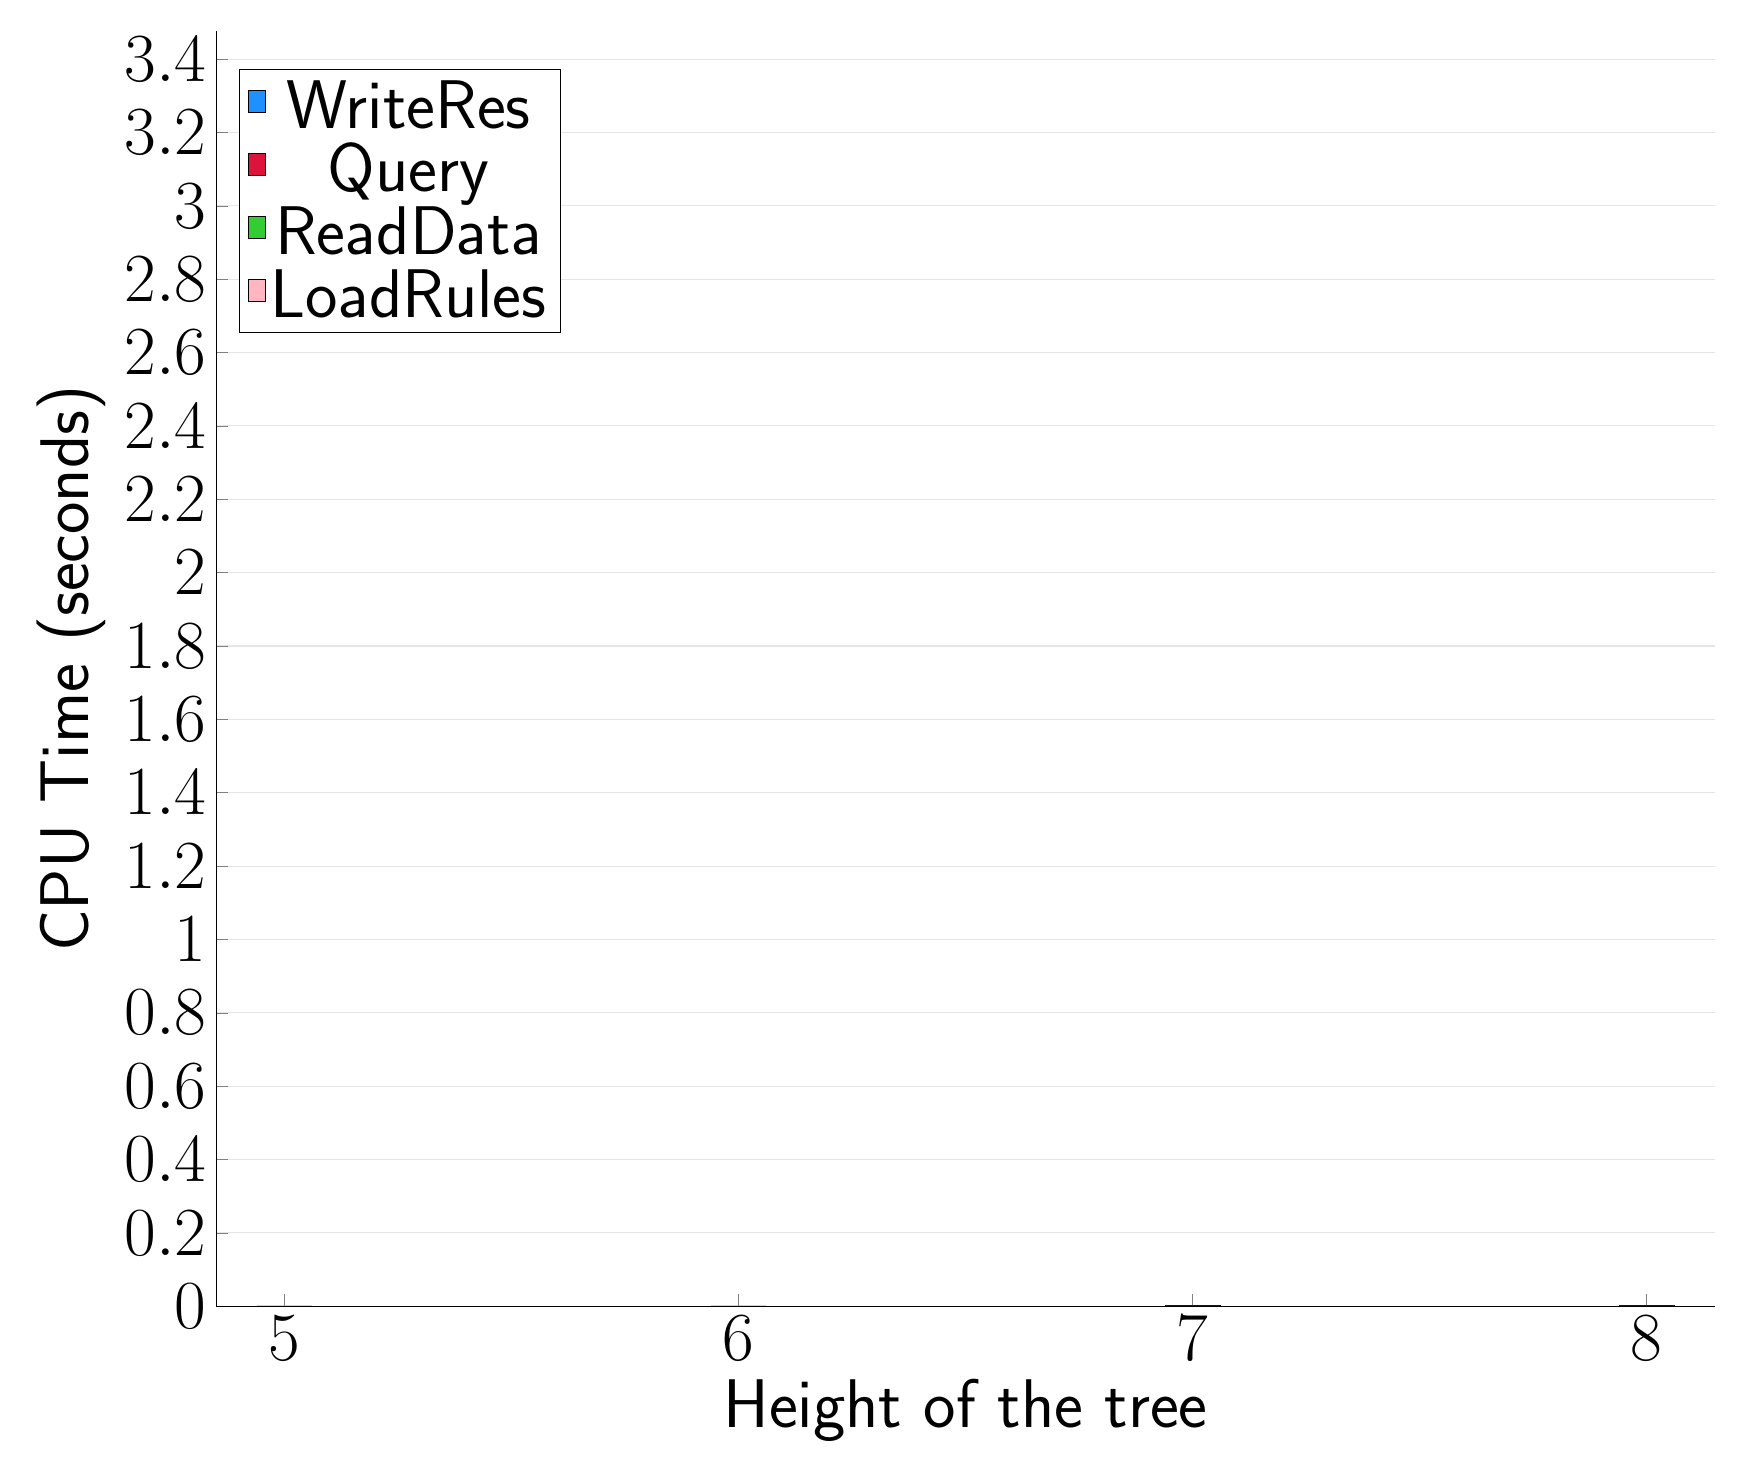
\begin{tikzpicture}
\begin{axis}[
   ybar stacked,
   width=1.7\textwidth,
   bar width=0.7cm,
   ymajorgrids, tick align=inside,
   major grid style={draw=gray!20},
   xtick=data,
   ymin=0, ymax=3.477,
   axis x line*=bottom,
   axis y line*=left,
   enlarge x limits=0.05,
   legend style={
       at={(0.23, 0.97)},
       anchor=north east,
       legend columns=1,
       font=\Huge,
   },
   ylabel={CPU Time (seconds)},
   xlabel={Height of the tree},
   label style={font=\Huge},
   tick label style={font=\Huge},
]
\addlegendimage{fill=DodgerBlue, draw=black, line width=0.2pt}
\addlegendentry{WriteRes}
\addlegendimage{fill=Crimson, draw=black, line width=0.2pt}
\addlegendentry{Query}
\addlegendimage{fill=LimeGreen, draw=black, line width=0.2pt}
\addlegendentry{ReadData}
\addlegendimage{fill=LightPink, draw=black, line width=0.2pt}
\addlegendentry{LoadRules}
\addplot +[fill=LightPink, draw=black, line width=0.2pt] coordinates {
(5, 0.0006482000000000001)
(6, 0.0006023000000000003)
(7, 0.0006140000000000001)
(7, 0.0006172999999999997)
(7, 0.0006282999999999998)
(8, 0.0006067999999999997)
(8, 0.0006163)
(8, 0.0006037000000000002)
};
\addplot +[fill=LimeGreen, draw=black, line width=0.2pt] coordinates {
(5, 0.0001656000000000008)
(6, 0.00018409999999999979)
(7, 0.0002479000000000005)
(7, 0.00024650000000000003)
(7, 0.0002437000000000006)
(8, 0.00034750000000000037)
(8, 0.0003618999999999993)
(8, 0.00036130000000000027)
};
\addplot +[fill=Crimson, draw=black, line width=0.2pt] coordinates {
(5, 2.909999999999925e-05)
(6, 4.959999999999997e-05)
(7, 0.00010279999999999979)
(7, 0.00010360000000000005)
(7, 0.0001047999999999999)
(8, 0.0002151000000000001)
(8, 0.00022010000000000028)
(8, 0.00021389999999999972)
};
\addplot +[fill=DodgerBlue, draw=black, line width=0.2pt] coordinates {
(5, 0.00016390000000000084)
(6, 0.0003033000000000003)
(7, 0.0006450000000000001)
(7, 0.0006495999999999999)
(7, 0.0007010999999999999)
(8, 0.0014631)
(8, 0.0014464999999999997)
(8, 0.0014653000000000005)
};
\end{axis}
\end{tikzpicture}

\end{document}
